\documentclass[12pt]{article}

\usepackage{amsmath,amsthm}
\usepackage{amsfonts}
\usepackage[psamsfonts]{amssymb}
\usepackage{palatino,euler} 
\usepackage[applemac]{inputenc}
\usepackage[french]{babel}
\usepackage[T1]{fontenc}
\usepackage{graphicx}
% \usepackage{tikz}
\usepackage{hyperref}


\setlength{\topmargin}{0pt}
\setlength{\headheight}{0pt}
\setlength{\headsep}{0pt}
\setlength{\textheight}{612pt}
\setlength{\textwidth}{400pt}
\setlength{\marginparwidth}{0pt}
\setlength{\oddsidemargin}{36pt}
\setlength{\parskip}{\baselineskip}
% \setlength{\parindent}{0pt}


\begin{document}

\noindent{\bf \large MAT 1460 : devoir 4 - Estimation de la vitesse atteinte}


\medskip
\noindent{\bf \'Equipe :} David Boucher-Roy, Thanh Huynh, David Grenier, Philip Higgins
\noindent{\bf Date} : \today

\bigskip


\bigskip

\hrule height0.3pt

\bigskip


\noindent{\bfseries 1. Vitesse terminale \`a l'altitude $x$ donn\'ee:}

\noindent
On cherche \`a obtenir la $v(t)$ vitesse terminale, une constante, en fonction de $x(t)$ ce qui entra\^ine une acc\'el\'eration nulle:
\begin{align*}
    0 = v'(t) &= -g(x(t)) + \frac1{2m}\rho(x(t)) C_D A v(t)^2\\
    v(t) &= \sqrt{\frac{2mg(x(t))}{\rho(x(t)) C_D A}}\\
    v(x) &= \sqrt{\frac{2mg(x)}{\rho(x) C_D A}}
\end{align*}

\bigskip

\hrule height0.3pt

\bigskip

\noindent{\bfseries 2. Utiliser des constantes pour les coefficients:}

\noindent
Il suffit de choisir des constantes appropri\'es pour $g$, l'acc\'el\'eration gravitationnelle terrestre, ainsi que $\rho$, la densit\'e de l'air lors du saut.
La force gravitationnelle est inversement proportionnelle au carr\'e de la distance entre les deux objets.
Le rayon moyen terrestre \'etant de 6371 km, le saut de Baumgartner varie d'environ $39km$ \`a $24km$ \`a l'ouverture du parachute. On calcule la contribution de l'altitude du saut sur la dite constante:
\[ \frac{(r_{terre} + alt_{max})^2}{r_{terre}^2} = \frac{(6371 + 39)^2}{6371^2} = 1.01248 \]

Puisque cette contribution est de $1.248\%$, on va donc assumer que l'altitude est n\'egligeable (dans cet exemple) sur l'acceleration gravitationnelle et prendre $g = 9.8065$ qui est approximativement celle de surface.

Pour $\rho$ la densit\'e de l'air, une constante raisonnable facile \`a obtenir est la densit\'e moyenne des 11 entr\'ees fournies:
\[ \rho = \frac1{11}\sum_{\rho_i}^{11} \rho_i = 0.0180915 \]

En substituant ces valeurs dans la solution analytique diff\'erentielle, Math\'ematica nous donne les \'equations $x(t)$ de la position et $v(t)$ de la vitesse:
\begin{align*}
    x(t) &= 47821.8 + 341.057 t - 11861.5 \ln(1 + e^{0.0575066t})\\
    v(t) &= -\frac{341.057(-1 + e^{0.0575066t})}{1 + e^{0.0575066t}}
\end{align*}

\noindent
On obtient les r\'esultats suivants:
\begin{figure}[h]
    \centering
    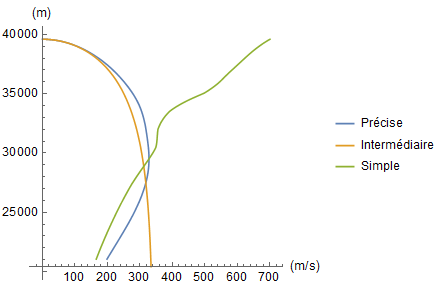
\includegraphics{AltitudeVsVitesse.png}\\
    \caption{Mod\`eles 1 \`a 3 - vitesse vs altitude.}
\end{figure}

\clearpage

\begin{table}[h]
    \centering
    \begin{tabular}{|l|r|r|}\hline
        M\'ethode &Altitude (km) &Vitesse (km/h)\\\hline
        Simple &39.600 &2522.84\\\hline
        Interm\'ediare &21.053 &1203.38\\\hline
        Pr\'ecise &29.513 &1180.90\\\hline
    \end{tabular}\\
    \caption{$V_{max}$ et altitude pour chacune des m\'ethodes.}
\end{table}

Nous observons que la m\'ethode simple repr\'esente mal le fait qu'une chute libre ne d\'ebute jamais \`a la vitesse terminale.
Toutefois la m\'ethode approxime bien les donn\'ees empiriques une fois que le parachutiste atteint sa vitesse maximale.

La m\'ethode interm\'ediaire est une bonne approximation en d\'ebut de chute, mais elle devient inexacte lorsque la vitesse est \'elev\'ee et que la densit\'e de l'air devient un facteur dominant.
En effet l'approximation de $\rho$ par la moyenne des donn\'ees est inf\'erieure \`a la densit\'e r\'eelle lorsqu'on atteint la vitesse maximale lors de la chute.

La solution diff\'erentielle num\'erique est \'evidemment celle la plus proche des donn\'ees recueillies lors du saut de Baumgartner.
Par contre, contrairement aux deux autres m\'ethodes, celle-ci fonctionne uniquement si on obtient des donn\'ees empiriques et ne nous permet pas d'extrapoler.

\end{document}

